\documentclass[10pt]{beamer}
\usetheme{Darmstadt}
\usepackage[utf8]{inputenc}
\usepackage{amsmath}
\usepackage{amsfonts}
\usepackage{amssymb}
\usepackage{graphicx}
\usepackage{tikz}
\usepackage{textpos}
\usepackage{ulem}
\usefonttheme{professionalfonts} % using non standard fonts for beamer
\setbeamertemplate{headline}{}
\setbeamertemplate{navigation symbols}{}
\setbeamertemplate{footline}{}

% COLORES 
\definecolor{pantone}{RGB}{50,98,149}
\definecolor{azuloscuro}{RGB}{48,58,187}
\definecolor{rojo}{RGB}{237,28,36}
\definecolor{negro}{RGB}{26,29,26}
\definecolor{palesilver}{RGB}{193,189,179}
\definecolor{blackcoffee}{RGB}{56,48,46}
\definecolor{AlmeriaBackground}{RGB}{193,189,179}
\definecolor{deepspacesparkle}{RGB}{79,99,103}
\definecolor{beige}{RGB}{238,245,219}
\definecolor{orangeredcrayola}{RGB}{254,95,85}
\definecolor{oldburgundy}{RGB}{65,39,34}
\definecolor{burgundy}{RGB}{114,17,33}
\definecolor{richblack}{RGB}{0,16,17}
\definecolor{middlered}{RGB}{215,129,106}
\definecolor{gray}{RGB}{191,191,191}
\definecolor{honeyellow}{RGB}{242,175,41}
\definecolor{flame}{RGB}{211,97,53}
\definecolor{gainsboro}{RGB}{223,223,223}
\definecolor{silvermetalic}{RGB}{164,165,174}

% ITEMS
\setbeamertemplate{itemize item}[circle]
\setbeamercolor{itemize item}{fg=burgundy}
\setbeamercolor{item projected}{bg=pantone, fg=white}
\setbeamertemplate{enumerate items}[circle]

% UNDERLINE

\newcommand\reduline{\bgroup\markoverwith{\textcolor{burgundy}{\rule[-0.5ex]{2pt}{1pt}}}\ULon}

\setbeamercolor{frametitle}{fg=white,bg=pantone}
\setbeamercolor{normal text}{fg=richblack}
\setbeamercolor{block title}{bg=burgundy}
\setbeamercolor{section in toc}{fg=burgundy}

\setlength{\TPHorizModule}{1cm} % horizontal unit
\setlength{\TPVertModule}{1cm} % vertical unit
\author{Jonathan Moreno Jiménez}
\title{Prueba Beamer}
%\setbeamercovered{transparent} 
%\setbeamertemplate{navigation symbols}{} 
%\logo{} 
%\institute{} 
%\date{} 
%\subject{}
\setbeamercovered{}
\newcommand{\director}{Directed by:\\Director name}

\author[Jonathan Moreno Jiménez]{\large Jonathan Moreno Jiménez  \\ \textcolor{white}{a} \\ \small Tutor: José A. Torres Arriaza}
\title[Trabajo fin de grado]{Estudio e implementación de un servicio de análisis de sentimientos para una tienda electrónica}
\date{10 de septiembre de 2020}
%\institute[UAL]{
%		Universidad de Almería \\ Escuela Superior de Ingeniería \\Grado en %Ingeniería Informática\\
%		\vspace{2mm}
%}

\begin{document}

\begin{frame}
\frametitle{Contenido}
\vspace{-5mm}
\hspace*{0.8cm}{\begin{minipage}[c][6cm]{0.5\textwidth}
\textbf{\tableofcontents}
\end{minipage}}
\vspace{5mm}
\begin{textblock}{5}(7,-4.25)
	
\includegraphics[width = 0.6\textwidth]{Figuras/negocios.png}
\end{textblock}
\end{frame}

\iffalse 
\begin{frame}
\frametitle{Contenido}
\begin{textblock}{5}(7,1.7)
	
\includegraphics[width = 0.6\textwidth]{Figuras/negocios.png}
\end{textblock}
\hspace*{0.5cm}{\begin{minipage}[c][6cm]{0.5\textwidth}
\begin{enumerate}
	\item \textbf{\textcolor{burgundy}{Introducción}}
	\vspace{1cm}
	\item \textbf{\textcolor{burgundy}{Solución propuesta}}
	\vspace{1cm}
	\item \textbf{\textcolor{burgundy}{Implementación}}
	\vspace{1cm}
	\item \textbf{\textcolor{burgundy}{Conclusiones}}
\end{enumerate}
\end{minipage}}
\end{frame}
\fi 


\section{Introducción}
\begin{frame}
\frametitle{Introducción}
\begin{figure}[htbp]
	\begin{center}
		\vspace{-1cm}
		{\large{\textbf{\textcolor{pantone}{\center Uso de servicios/soluciones de IA en Europa}}}}\par\medskip\medskip\medskip\medskip\medskip
		\includegraphics[width = .95\textwidth]{Figuras/AIuse}
	\end{center}
\end{figure}
\end{frame}

\section{Solución propuesta}
\begin{frame}
\frametitle{Solución propuesta}
\begin{textblock}{5}(9,-0.25)
	
\includegraphics[width = 0.4\textwidth]{Figuras/goal.png}
\end{textblock}
\begin{minipage}[c][3cm]{0.73\textwidth}
\textbf{\textcolor{burgundy}{Objetivo}}: Ilustrar el uso de la inteligencia artificial como herramienta de marketing digital. Se desarro-
llará un portal web donde se integrarán los siguientes servicios:
\vspace{.15cm}

\begin{itemize}
	\item Análisis de sentimientos
	\vspace{.15cm}
	\item Interfaz conversacional
\end{itemize}

\end{minipage}
\pause

\vspace{.5cm}
\begin{block}{Dirección de la tienda}
\url{https://wordpress-aek6a4275q-ew.a.run.app/}
\end{block}

\pause
\vspace{.5cm}

\begin{block}{Código de la aplicación}
\url{https://github.com/jo4nymj/sentiment-analysis}
\end{block}
\end{frame}


\begin{frame}
\frametitle{Tecnología y herramientas}
\vspace{-1.5cm}
\begin{columns}[T]
\begin{column}{0.33\textwidth}
   \begin{textblock}{1.75}(0.5,3.3)
		
\includegraphics[width =1\textwidth]{Figuras/technology.jpg}
	\end{textblock}
   \textbf{\textcolor{burgundy}{Tecnologías}}
   \begin{itemize}
   		\item GoLang
   		\item API REST
   		\item PHP
   		\item Contenedores
   \end{itemize} \pause
\end{column}
\hspace{-0.8cm}
\begin{column}{0.33\textwidth}
	\begin{textblock}{2}(0.5,5.7)
		
\includegraphics[width =1\textwidth]{Figuras/tools.png}
	\end{textblock}
     \textbf{\textcolor{burgundy}{Herramientas}}
    \begin{itemize}
   		\item Git
   		\item Github
   		\item Visual Studio Code
   		\item Trello
   		\item Postman
   		\item Wordpress + Plugins
   		\item Servicios de Google Cloud
   \end{itemize} \pause
\end{column}
\begin{column}{0.33\textwidth}
	\begin{textblock}{1.75}(0.7,4.8)
		
\includegraphics[width =1\textwidth]{Figuras/cloudicon.png}
	\end{textblock}
    \textbf{\textcolor{burgundy}{Google Cloud}}
    \begin{itemize}
    	\item Cloud SQL
   		\item Container Registry
   		\item Cloud Logging
   		\item Cloud Storage
   		\item NLP
   		\item Cloud Run
   		\item Dialogflow
   \end{itemize}
\end{column}
\end{columns}
\end{frame}

\begin{frame}
\frametitle{Tecnología y herramientas}
\framesubtitle{Natural Language Processing}
\begin{textblock}{1.25}(10,0.10)
	
\includegraphics[width = 1\textwidth]{Figuras/emoticonos.png}
\end{textblock}
\begin{textblock}{15}(0.2,0.5)
	\large \textbf{\textcolor{pantone}{Análisis de sentimientos realizado por NLP}}
\end{textblock}
\vspace{1.5cm}
\begin{figure}[htbp]
	\begin{center}
%		\large{\textbf{\textcolor{pantone}{Análisis de sentimientos realizado por NLP}}}\par\medskip\medskip\medskip\medskip
		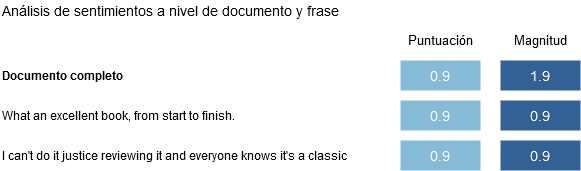
\includegraphics[width = .95\textwidth]{Figuras/puntuacion.png}
	\end{center}
%	\caption{\label{fig:NLP} Análisis de sentimientos realizado por NLP}
\end{figure}
\pause
\vspace{0.5cm}
\begin{figure}[htbp]
	\begin{center}
		
\includegraphics[width = .95\textwidth]{Figuras/estrellas.png}
	\end{center}
\end{figure}
\end{frame}

\begin{frame}
\frametitle{Tecnología y herramientas}
\framesubtitle{Dialogflow}
\begin{textblock}{1.5}(9.4,-2.6)
	
\includegraphics[width = 1\textwidth]{Figuras/robotico.png}
\end{textblock}
\begin{textblock}{15}(2.5,-2.4)
	\large \textbf{\textcolor{pantone}{Funcionamiento de Dialogflow}}
\end{textblock}

\begin{textblock}{13}(-1.25,-2.4)
	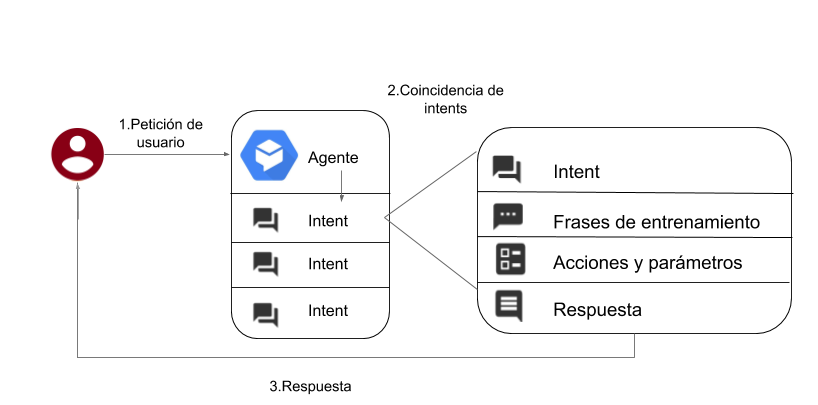
\includegraphics[width =1\textwidth]{Figuras/FlujoCoincidencias.png}
\end{textblock}
\end{frame}

\begin{frame}
\frametitle{Tecnología y herramientas}
\framesubtitle{Cloud Run}

\begin{textblock}{8}(8.8,2.2)
	
\includegraphics[width =0.30\textwidth]{Figuras/desarrollo-web}
\end{textblock}
\vspace{-0.2cm}
Se trata de una plataforma de computación \textbf{\textcolor{burgundy}{serverless}} que ejecuta \textbf{\textcolor{burgundy}{contenedores sin estado}}. \pause \vspace{0.8cm} \newline
\begin{beamercolorbox}[sep=0.6em,ht=1.6cm, wd=2.9cm,center,rounded=true,shadow=true]{block title}
\large ¿A qué nos referimos con serverless? 
\end{beamercolorbox} \vspace{1cm} \pause
\begin{textblock}{5}(3.7,-2.7)
\small Es un modelo de cloud computing donde el proveedor es el responsable de ejecutar el código mediante la asignación dinámica de recursos.
\end{textblock} \pause
\begin{beamercolorbox}[sep=0.6em,ht=1.6cm,wd=2.9cm,center,rounded=true,shadow=true]{block title}
\large ¿Qué son los contenedores sin estado?
\end{beamercolorbox} \pause
\begin{textblock}{5}(3.7,-1.9)
\small Los datos se almacenan fuera del contenedor. Si se modifican los ficheros durante el tiempo de ejecución los cambios no serán persistentes
\end{textblock}\end{frame}

\section{Implementación}
\begin{frame}
\frametitle{Arquitectura}
\vspace{-0.5cm}
\begin{figure}[htbp]
	\begin{center}
		\large{\textbf{\textcolor{pantone}{Arquitectura del sistema}}}\par\medskip\medskip\medskip\medskip
		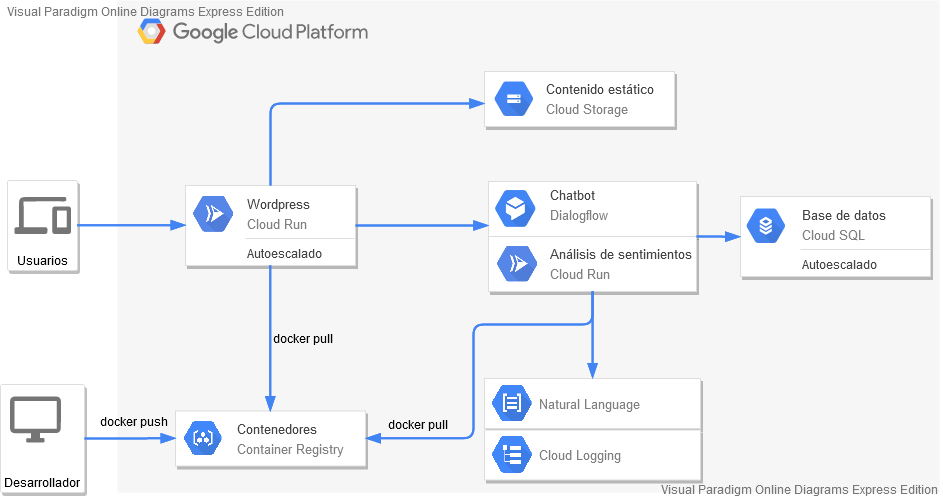
\includegraphics[width = 1\textwidth]{Figuras/ArquitecturaV3.png}
	\end{center}
%	\caption{\label{fig:Arquitectura} Arquitectura del sistema}
\end{figure}
\end{frame}

\begin{frame}
\frametitle{Aplicación de análisis de sentimientos}
\vspace{-1.5cm}
\begin{textblock}{15}(3.5,-2)
	\large{\textbf{\textcolor{pantone}{Modelo de la API}}}
\end{textblock}
\begin{textblock}{10.5}(-0.70,-0.75)
	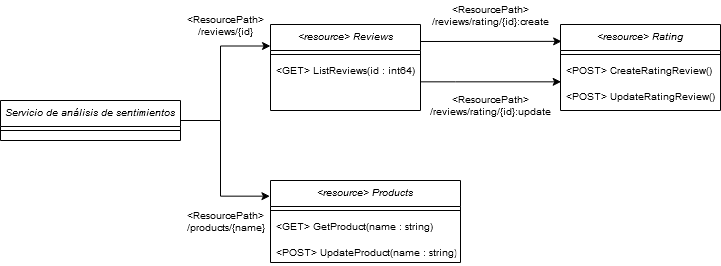
\includegraphics[width = 1.15\textwidth]{Figuras/ClassDiagram-Page-2.png}
\end{textblock}
	
\end{frame}

\begin{frame}
\frametitle{Aplicación de análisis de sentimientos}
\vspace{-1.5cm}
\begin{textblock}{15}(3.5,-2)
	\large{\textbf{\textcolor{pantone}{Modelo de la API}}}
\end{textblock}
\begin{textblock}{10.5}(-0.70,-1.15)
	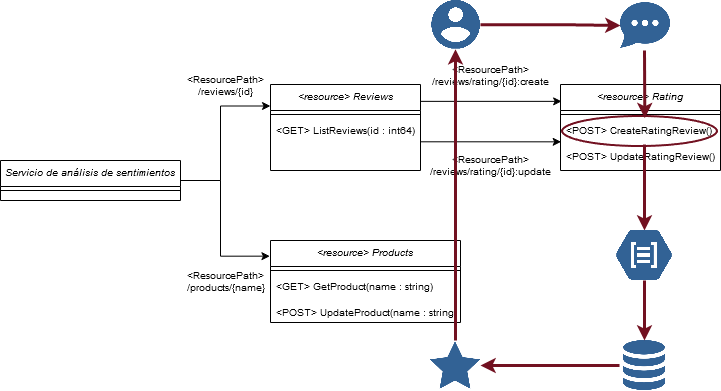
\includegraphics[width = 1.15\textwidth]{Figuras/API2.png}
\end{textblock}
	
\end{frame}

\section{Conclusiones}

\begin{frame}
\frametitle{Conclusiones}
%\vspace{-1cm}
\begin{textblock}{2.5}(8.3,5.1)
	
\includegraphics[width = 1\textwidth]{Figuras/conclusions.png}
\end{textblock}
\begin{center}
    \begin{minipage}{\textwidth}
      \begin{enumerate}
        \item La computación en la nube es una herramienta con un gran potencial para las pymes. \vspace{0.6cm} \pause
        \item Cloud Run no es la plataforma más adecuada para alojar la página web. Pero sí es una solución que encaja con la aplicación de análisis de sentimientos. \vspace{0.6cm} \pause
        \item Se debe ajustar el método que discretiza la puntuación y usar la magnitud para eliminar ambigüedades. \vspace{0.6cm} \pause
		\item Es muy importante conectar el chatbot con \newline la base de datos. \vspace{0.5cm}
      \end{enumerate} 
    \end{minipage}
\end{center}
\end{frame}


\end{document}
